\begin{frame}[fragile]
  \frametitle{课程主旨}
  \begin{center}
  {\Huge 为“疯狂”点赞\\
    \vspace{0.5cm}
    为科学“正名”}\\
  \vspace{1cm}
  {\Large 正史书王迹,稗官言秘闻。\\
    \vspace{0.2cm}
    万般皆杳杳,唯有醉中真。}
\end{center}
\end{frame}

\begin{frame}
  \frametitle{科学}
  \begin{block}{科学(science)}
科学(science)的基本特征是其方法论:对世界的认识源于观测或实验的信息(或者数据),总结信息时会形成模型(亦称假说或理论),模型会指导进一步的探索,指导遇到这些模型无法解释的现象,这就导致对这些模型的更新和替代。这就是科学的方法。只有用科学的方法进行的探索才能称为科学。
  \end{block}
\end{frame}

\begin{frame}
  \frametitle{参考教材}
  \begin{figure}
    \centering
    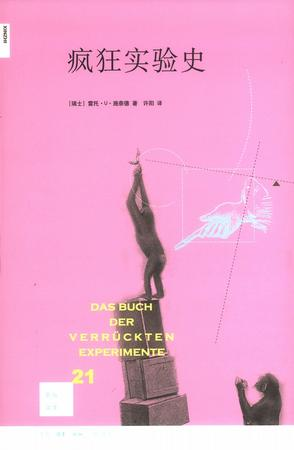
\includegraphics[width=5cm]{c0.book.01.jpg}
    \qquad
    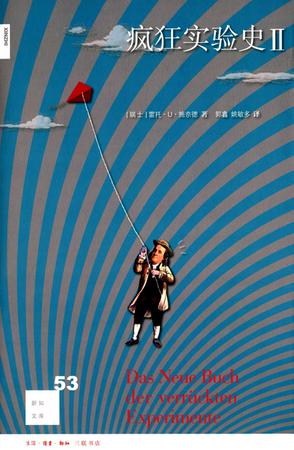
\includegraphics[width=5cm]{c0.book.02.jpg}
  \end{figure}
\end{frame}

\begin{frame}
  \frametitle{课外读物}
  \begin{figure}
    \centering
    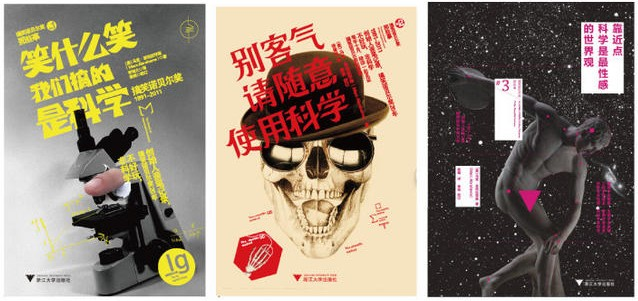
\includegraphics[width=11cm]{c0.book.03.jpg}
  \end{figure}
\end{frame}

\begin{frame}
  \frametitle{课外读物}
  \begin{figure}
    \centering
    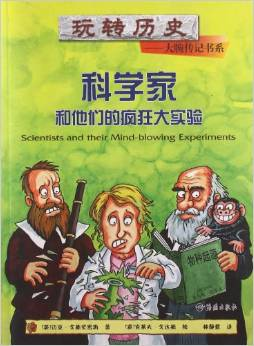
\includegraphics[width=2.7cm]{c0.book.04.jpg}\quad
    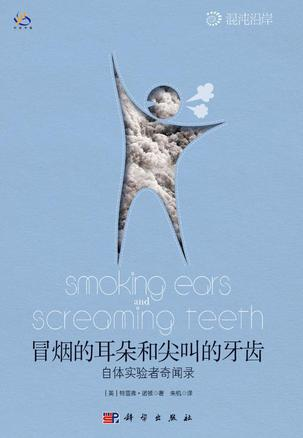
\includegraphics[width=2.55cm]{c0.book.05.jpg}\quad
    
\includegraphics[width=2.8cm]{c0.book.06.jpg}\\
    
\includegraphics[width=2.8cm]{c0.book.07.jpg}\hspace{1cm}
    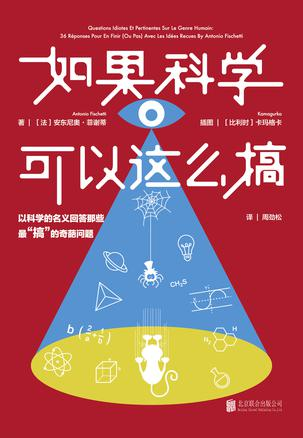
\includegraphics[width=2.8cm]{c0.book.08.jpg}
  \end{figure}
\end{frame}

\begin{frame}
  \frametitle{授课资料}
  \begin{figure}
    \centering
    
\includegraphics[width=0.55\textwidth]{qr.png}
  \end{figure}
  \begin{center}
  \href{https://github.com/Yixf-Education/course_Crazy_Experiment}{https://github.com/Yixf-Education/course\_Crazy\_Experiment}
  \end{center}
\end{frame}

\begin{frame}
  \frametitle{课程安排}
  \begin{center}
  \alert{前8(9)周,每周二,晚上两节(18:00-20:00),西楼402}\\
  \vspace{0.2cm}
  \end{center}
  \begin{block}{授课内容}
    \begin{itemize}
      \item 物理学、化学、心理学、生物学、医学、……
      \item 谈天说地,评古论今
    \end{itemize}
  \end{block}
\end{frame}

\begin{frame}
  \frametitle{\alert{考核方式}}
  \begin{block}{考勤}
    \begin{itemize}
      \item 不点名,但随机提问
      \item 缺勤0次——优秀(及以下)
      \item 缺勤1次——良好(及以下)
      \item 缺勤2次——及格(及以下)
      \item 缺勤3次——不及格
    \end{itemize}
  \end{block}
  \pause
  \begin{block}{报告}
    \begin{itemize}
      \item 内容:自己关于某个(疯狂)实验的简单设想
      \item 要求:电子版,~500字(一页纸),含灵感来源、实验目的、基本方案等
      \item 提交:yixfbio@gmail.com,课程名-学号-姓名-共享/保密.doc
      \item 抄袭——不及格
    \end{itemize}
  \end{block}
\end{frame}

